\chapter{The concept of black hole 2: The global view}
\label{s:glo}

\minitoc

\section{Introduction}

Having attempted in Chap.~\ref{s:def} to characterize a black hole by the local
properties of its boundary, we turn now to the general definition of a black
hole. As it could have been anticipated from the naive ``definition'' given
in Sec.~\ref{s:def:first_defin}, the mathematically meaningful definition
of a black hole cannot be local: it has to take into account the full
spacetime structure, in particular its future asymptotics. Indeed, to decide
whether a null geodesic can escape or not, one has to wait until the ``end
of time'' to conclude.

In this chapter, we therefore consider the global spacetime picture to
arrive at the definition of a black hole. This amounts to focus on the
spacetime asymptotics (the region where the ``distant observers'' live), which
is described by introducing a conformal completion of spacetime.

%%%%%%%%%%%%%%%%%%%%%%%%%%%%%%%%%%%%%%%%%%%%%%%%%%%%%%%%%%%%%%%%%%%%%%%%%%%%%%%%%%%%%%%%

\section{Conformal completion}

In order to define an asymptotical flat spacetime as a spacetime that ressembles
Minkowski spacetime in the region ``far from the massive bodies'',  we shall
investigate first the asymptotics of Minkowski spacetime by performing some
conformal completion of it.

\subsection{Compactified coordinates on Minkowski spacetime}

In this section $(\M,\w{g})$ is the 4-dimensional Minkowski spacetime,
i.e. $\M$ is a smooth manifold diffeomorphic to $\mathbb{R}^4$ and $\w{g}$
is the metric tensor whose expression in terms of the global coordinates
$(x^\alpha) = (t, x, y, z)$ implementing the diffeomorphism to $\mathbb{R}^4$
(i.e. the so-called \defin{Minkowskian coordinates}\index{Minkowskian!coordinates})
is
\be
    g_{\mu\nu} \D x^\mu \D x^\nu = - \D t^2 + \D x^2 + \D y^2 + \D z^2 .
\ee
Since we have to deal with the ``far'' region, it is natural to introduce
$r := \sqrt{x^2+y^2+z^2}$ and the associated spherical coordinates
$(x^\alpha) = (t,r,\th,\ph)$, which are related to the Minkowskian coordinates
by
\be
    \left\{ \begin{array}{l}
    x = r\sin\th\cos\ph \\
    y = r\sin\th\sin\ph \\
    z = r\cos\th .
    \end{array} \right.
\ee
The coordinates $(t, r,\th,\ph)$ span
$\mathbb{R}\times(0,+\infty)\times (0,\pi) \times (0,2\pi)$ and do not cover
the whole manifold $\M$ as a regular chart (cf. Sec.~\ref{s:bas:def_manif} of Appendix~\ref{s:bas}), but $\M\setminus \Pi$, where $\Pi$ is the closed half hyperplane defined
by $y=0$ and $x\geq 0$. Once expressed in terms of the
spherical coordinates, the Minkowski metric takes the form
\be
    g_{\mu\nu} \D x^\mu \D x^\nu = - \D t^2 + \D r^2
        + r^2 \left( \D\th^2 + \sin^2\th \, \D\ph^2 \right) .
\ee

\begin{figure}
\centerline{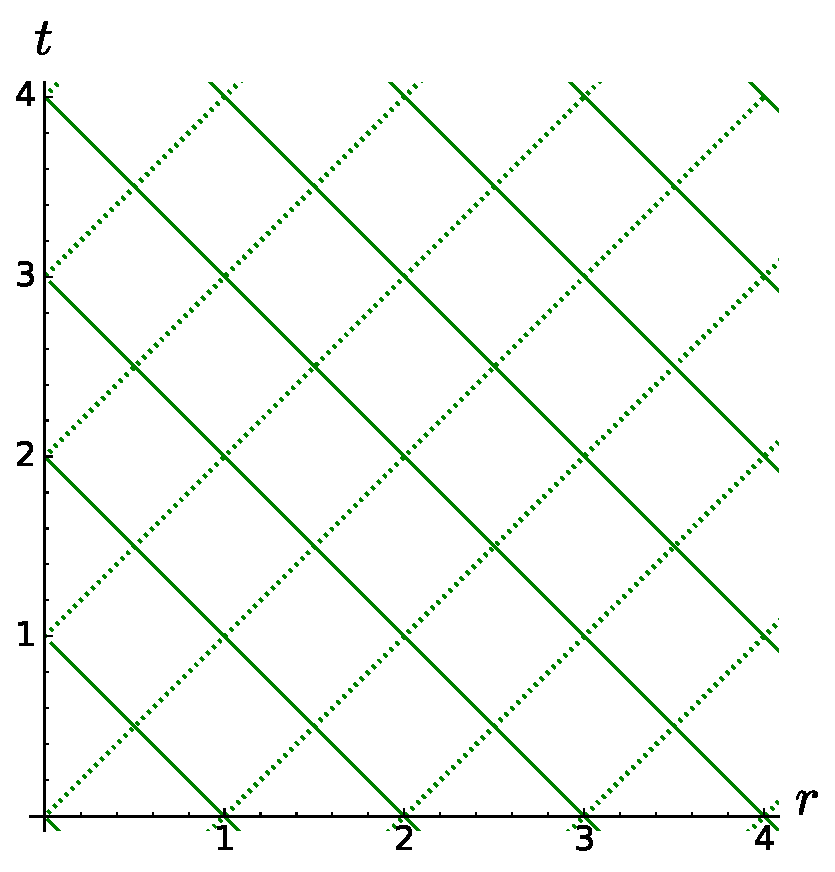
\includegraphics[width=0.5\textwidth]{glo_null_coord.pdf}}
\caption[]{\label{f:glo:glo_null_coord} \footnotesize
Lines of constant null coordinates $u$ (dashed) and $v$
(solid) in terms of the coordinates $(t,r)$.}
\end{figure}


Let us introduce the null coordinate system $(u,v,\th,\ph)$ where $u$ and
$v$ are respectively the retarted\index{retarted!time} and advanced\index{advanced!time}
time defined by (cf. Fig.~\ref{f:glo:glo_null_coord})
\be \label{e:glo:advanced_retarded}
    \left\{ \begin{array}{l}
    u = t - r\\
    v = t + r
    \end{array} \right.
    \iff
    \left\{ \begin{array}{l}
    t = \frac{1}{2} (v+u)\\[1ex]
    r = \frac{1}{2} (v-u) .
    \end{array} \right.
\ee
The metric tensor takes then the shape
\be
    g_{\mu\nu} \D x^\mu \D x^\nu = - \D u \, \D v
        + \frac{1}{4} (v-u)^2 \left(  \D\th^2 + \sin^2\th \, \D\ph^2 \right) .
\ee
The coordinates $(u,v)$ span the half part of $\mathbb{R}^2$ defined by
$u<v$. In order to have coordinates in a finite range, let us consider
their arctangents (cf. Fig.~\ref{f:glo:glo_atan})
\be
    \left\{ \begin{array}{l}
    U = \arctan u \\
    V = \arctan v .
    \end{array} \right.
\ee
Then $(U,V)$ span the half part of $(-\pi/2, \pi/2)\times (-\pi/2, \pi/2)$
defined by $U < V$
(since $\mathrm{atan}$ is a monotonically increasing function, cf. Fig.~\ref{f:glo:glo_atan}):
\be \label{e:glo:span_UV}
    -\frac{\pi}{2} < U < \frac{\pi}{2}, \quad
    -\frac{\pi}{2} < V < \frac{\pi}{2}, \quad\mbox{and}\quad U < V.
\ee

\begin{figure}
\centerline{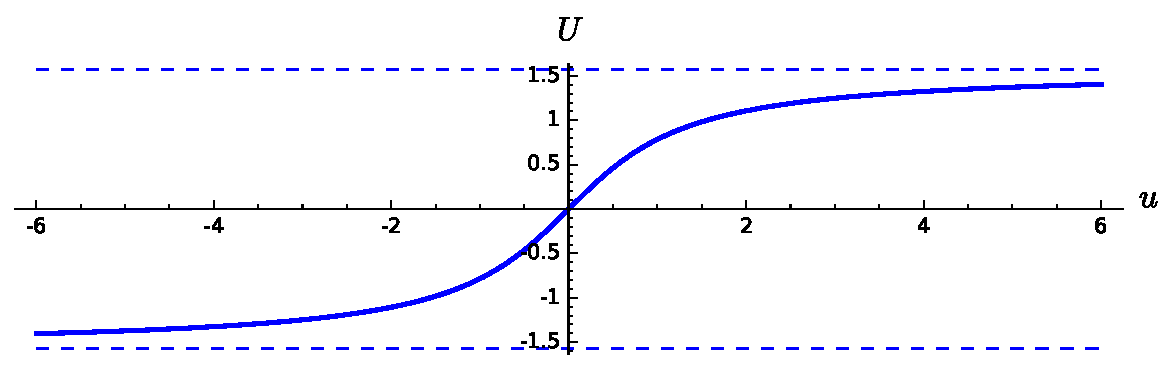
\includegraphics[width=0.8\textwidth]{glo_atan.pdf}}
\caption[]{\label{f:glo:glo_atan} \footnotesize
The arctangent function mapping $\mathbb{R}$ to $(-\pi/2, \pi/2)$.}
\end{figure}

In terms of the coordinates $(x^\alpha)=(U,V,\th,\ph)$, the Minkowski
metric becomes\footnote{Cf. Sec.~\ref{s:sam:worksheets} for
the computation.}:
\be \label{e:glo:g_UV}
    g_{\mu\nu} \D x^\mu \D x^\nu = \frac{1}{4\cos^2 U \cos^2 V}
    \left[ - 4 \D U \, \D V + \sin^2(V-U) \left(  \D\th^2 + \sin^2\th \, \D\ph^2 \right)
    \right] .
\ee

\subsection{Conformal metric}

In the right-hand side of (\ref{e:glo:g_UV}) there appears clearly the metric
$\w{\tilde{g}}$ defined by
\be \label{e:glo:tilde_g_Omega}
    \encadre{ \w{\tilde{g}} = \Omega^2 \w{g} } ,
\ee
where $\Omega$ is the scalar field $\M \rightarrow \mathbb{R}$ defined by
\begin{subequations}
\begin{align}
    \Omega & =  2 \cos U \cos V \label{e:glo:Omega_UV} \\
           & =  \frac{2}{\sqrt{1+u^2}\sqrt{1+v^2}} \label{e:glo:Omega_uv}\\
           & =  \frac{2}{\sqrt{(t-r)^2+1}\sqrt{(t+r)^2+1}} . \label{e:glo:Omega_tr}
\end{align}
\end{subequations}
We notice on (\ref{e:glo:Omega_uv}) and (\ref{e:glo:Omega_tr}) that the function
$\Omega$ never vanishes on $\M$, so that the bilinear form $\w{\tilde{g}}$ defined by
(\ref{e:glo:tilde_g_Omega}) constitutes a well behaved metric on $\M$.
Moreover, since $\Omega^2 > 0$, $\w{\tilde{g}}$ has the same signature as
$\w{g}$, i.e. $(-,+,+,+)$.
The specific expression of $\w{\tilde{g}}$ is deduced from (\ref{e:glo:g_UV})
and (\ref{e:glo:Omega_UV}):
\be \label{e:glo:tg_UV}
    \tilde{g}_{\mu\nu} \D x^\mu \D x^\nu =  - 4 \D U \, \D V
        + \sin^2(V-U) \left(  \D\th^2 + \sin^2\th \, \D\ph^2 \right) .
\ee

In view of (\ref{e:glo:tilde_g_Omega}), one says that the metric $\w{\tilde{g}}$
is \defin{conformal to}\index{conformal} the metric $\w{g}$, or equivalently,
that the metrics $\w{g}$ and $\w{\tilde{g}}$ are
\defin{conformally related}\index{conformally related metrics},
or that $\w{\tilde{g}}$ arises from $\w{g}$ via a
\defin{conformal transformation}\index{conformal!transformation}.

A key property of a conformal transformation is to preserve the orthogonality
relations, since (\ref{e:glo:tilde_g_Omega}) clearly
implies, at any point $p\in\M$,
\[
    \forall (\w{u},\w{v})\in T_p\M\times T_p\M,\quad
    \w{\tilde{g}}(\w{u},\w{v}) = 0 \iff \w{g}(\w{u},\w{v}) = 0 .
\]
In particular, a null vector for $\w{g}$ remains a null vector for $\w{\tilde{g}}$:
\[
    \forall \wl \in T_p\M,\quad
    \w{\tilde{g}}(\wl,\wl) = 0 \iff \w{g}(\wl,\wl) = 0 .
\]
Consequently the light cones of $(\M,\w{g})$ and $(\M,\w{\tilde{g}})$
are identical.
Moreover, since $\Omega^2>0$, the spacelike and timelike characters of vectors
is preserved as well:
\be
    \begin{array}{ll}
    \forall \w{v} \in T_p\M,\ &
        \w{v} \mbox{\ spacelike for\ } \w{\tilde{g}} \iff \w{v} \mbox{\ spacelike for\ } \w{g} \\
    & \w{v} \mbox{\ timelike for\ } \w{\tilde{g}} \iff \w{v} \mbox{\ timelike for\ } \w{g} .
    \end{array}
\ee
It follows that a curve $\Li$ is timelike (resp. null, spacelike) for $\w{\tilde{g}}$
iff $\Li$ is timelike (resp. null, spacelike) for $\w{g}$. Similarly,
a hypersurface $\Sigma$ is timelike (resp. null, spacelike) for $\w{\tilde{g}}$
iff $\Li$ is timelike (resp. null, spacelike) for $\w{g}$.

What about geodesics? Let us first recall that a null curve is not necessarily
a null geodesic (cf. Remark~\ref{r:def:null_curves} on page~\pageref{r:def:null_curves}),
so that one cannot deduce from the above results that conformal transformations
preserve null geodesics. Actually, this turns out to be true:
\begin{quote}
A smooth curve $\Li$ in $\M$ is a null geodesic for $\w{\tilde{g}}$ iff
$\Li$ is a null geodesic for $\w{g}$.
\end{quote}
To prove it, it suffices to write explicitly the geodesic equation
and to express the Christoffel symbols of $\w{\tilde{g}}$ in terms of those
of $\w{g}$ and the derivatives of $\Omega$ (see e.g. Appendix~D of Wald's
textbook \cite{Wald84} for details).

On the contrary conformal transformations preserve neither the timelike
geodesics nor the spacelike ones.

The coordinates $(U,V)$ are of null type; let us consider instead
the ``time+space'' coordinates $(\tau,\chi)$ defined by\footnote{Notice the
similarity with (\ref{e:glo:advanced_retarded}) up to some $1/2$ factors.}
\be \label{e:glo:tau_chi_U_V}
    \left\{ \begin{array}{l}
    \tau = V + U \\
    \chi = V - U
    \end{array} \right.
    \iff
    \left\{ \begin{array}{l}
    U = \frac{1}{2} (\tau - \chi) \\[1ex]
    V = \frac{1}{2} (\tau + \chi)
    \end{array} \right.
\ee
Given (\ref{e:glo:span_UV}), the range of these new coordinates is
\be
    0 < \chi < \pi \quad\mbox{and}\quad
    \chi - \pi < \tau < \pi - \chi .
\ee
In other words, if we draw the Minkowski spacetime in the $(\tau,\chi)$ plane,
it takes the shape of a half-diamond: see Fig.~\ref{f:glo:glo_conf_diag_Mink}.

\begin{figure}
\centerline{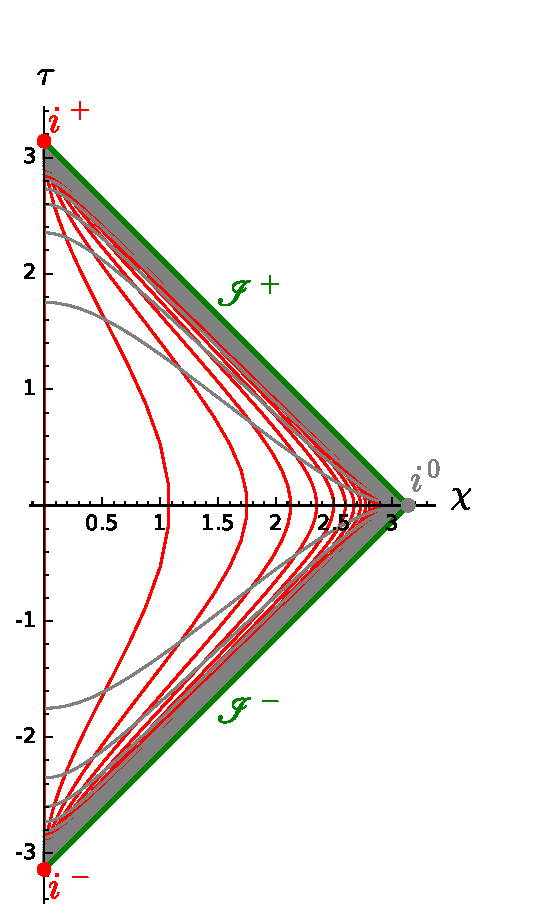
\includegraphics[width=0.5\textwidth]{glo_conf_diag_Mink.pdf}}
\caption[]{\label{f:glo:glo_conf_diag_Mink} \footnotesize
Conformal diagram of Minkowski spacetime. Constant-$r$ curves are drawn in
red, while constant-$t$ ones are drawn in grey.}
\end{figure}

The expression of the conformal metric in terms of the coordinates
$(x^\alpha) = (\tau,\chi,\th,\ph)$ is deduced from that in terms of
$(U,V,\th,\ph)$ as given by (\ref{e:glo:tg_UV}):
\be
    \tilde{g}_{\mu\nu} \D x^\mu \D x^\nu =  - \D\tau^2
        + \D \chi^2
        + \sin^2\chi \left(  \D\th^2 + \sin^2\th \, \D\ph^2 \right) .
\ee
On a $\tau = \mathrm{const}$ hypersurface, i.e. setting $\D\tau=0$,
we recognize the metric of the hypersphere
$\mathbb{S}^3$ in standard hyperspherical coordinates $(\chi,\th,\ph)$.

On the other side, the expression of the conformal factor in the
coordinates $(\tau,\chi,\th,\ph)$ is easily deduced from
(\ref{e:glo:Omega_UV}) and
(\ref{e:glo:tau_chi_U_V}):
\be
    \Omega = \cos\tau + \cos\chi .
\ee

\subsection{Conformal completion of Minkowski spacetime}


\subsection{Asymptotic flatness}

%%%%%%%%%%%%%%%%%%%%%%%%%%%%%%%%%%%%%%%%%%%%%%%%%%%%%%%%%%%%%%%%%%%%%%%%%%%%%%%%%%%%%%%%

\section{General definition of a black hole}

%%%%%%%%%%%%%%%%%%%%%%%%%%%%%%%%%%%%%%%%%%%%%%%%%%%%%%%%%%%%%%%%%%%%%%%%%%%%%%%%%%%%%%%%

\section{Stationary black holes}

Hawking's strong rigity theorem
